\documentclass{beamer}
\usepackage[utf8]{inputenc}
\usepackage{graphicx}
\usetheme{Warsaw}
\usecolortheme{seahorse}

\title{Genalice/SciLifeLab NGI Applications - indels in NA12878 }
\author{Szilveszter Juhos, Erik Borgström, Max Käller}
\institute{SciLifeLab}
\date{6th Oct. 2016 }
\begin{document}
\frame{\titlepage}
			  
\begin{frame}
	\frametitle{NA12878 truth set, using only NIST high confidence regions}
	\begin{block}{Platinum reads from Illumina (NA12878 ERR194147) }
		GIAB calls are considered as reference, only insertions and deletions extracted
	\end{block}
	\begin{block}{Focus on missing calls (those that are in the GIAB/NIST truth set, but not in the GA call set)}
		Two methods: direct calls by gaVariant and population calls, visualized in IGV
	\end{block}
\end{frame}

\begin{frame}
	\frametitle{Insertion / deletion ratios}
	\begin{table}[]
		\centering
		\caption{Indel ratios}
		\label{indelratios}
		\begin{tabular}{lll}
			method          & ins/del ratio & ins/del bases \\
			gaVariant       & 0.953265      & 0.755639      \\
			population call & 0.906097      & 0.680871      \\
			truth set       & 1.00812       & 0.93672      
		\end{tabular}
	\end{table}

	\begin{table}[]
		\centering
		\caption{Missing indels}
		\label{missingindels}
		\begin{tabular}{lll}
										& missing inserts & missing deletions \\
										gaVariant       & 8115            & 5441              \\
										population call & 14832           & 10056            
		\end{tabular}
	\end{table}
\end{frame}

\begin{frame}
	\begin{block}{Ins/del ratios are much better for high confidence regions than was measured before.}
		\begin{itemize}
			\item Also, missing indels are usually in STRs - this can be a sequencing artefact, not real false negatives (see examples below)
			\item Many indels are missing simply because they were detected by other technology and not by processing the platinum read set
			\item VCF of missing calls attached
		\end{itemize}
	\end{block}
\end{frame}

\begin{frame}
\frametitle{Deletion size distribution}
\center{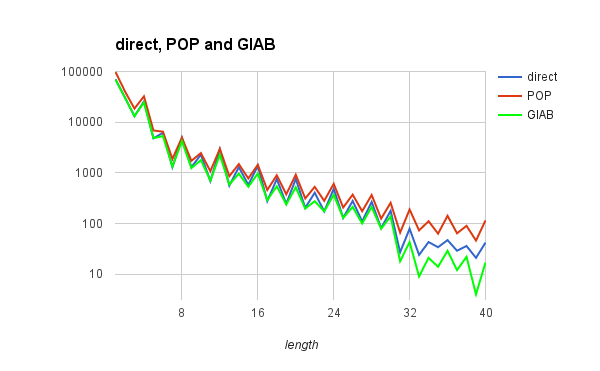
\includegraphics[width=1.0\linewidth]{deletions_bins.png}}
\end{frame}

\begin{frame}
\frametitle{Insert size distribution}
\center{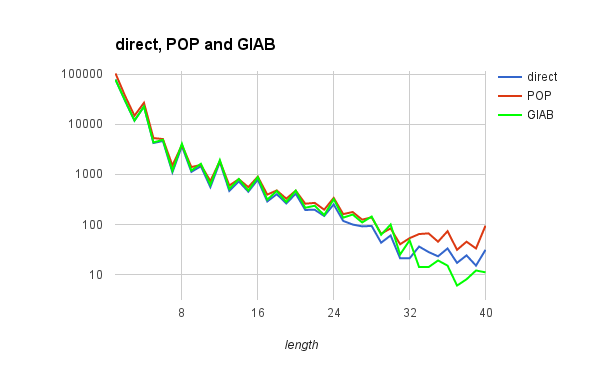
\includegraphics[width=1.0\linewidth]{inserts_bins.png}}
\end{frame}

\begin{frame}
\frametitle{IGV tracks}
	\begin{block}{IGV tracks}
		\begin{itemize}
			\item Upper alignment track: Genalice GAR
			\item Lower alignment track: BWA alignment
			\item GIAB truth set
			\item GA direct call by gaVariant
			\item GA population call 
			\item GA direct call - missing calls
			\item GA population call - missing calls
		\end{itemize}
	\end{block}
\end{frame}

\begin{frame}
\frametitle{Missing deletion in repeat}
\center{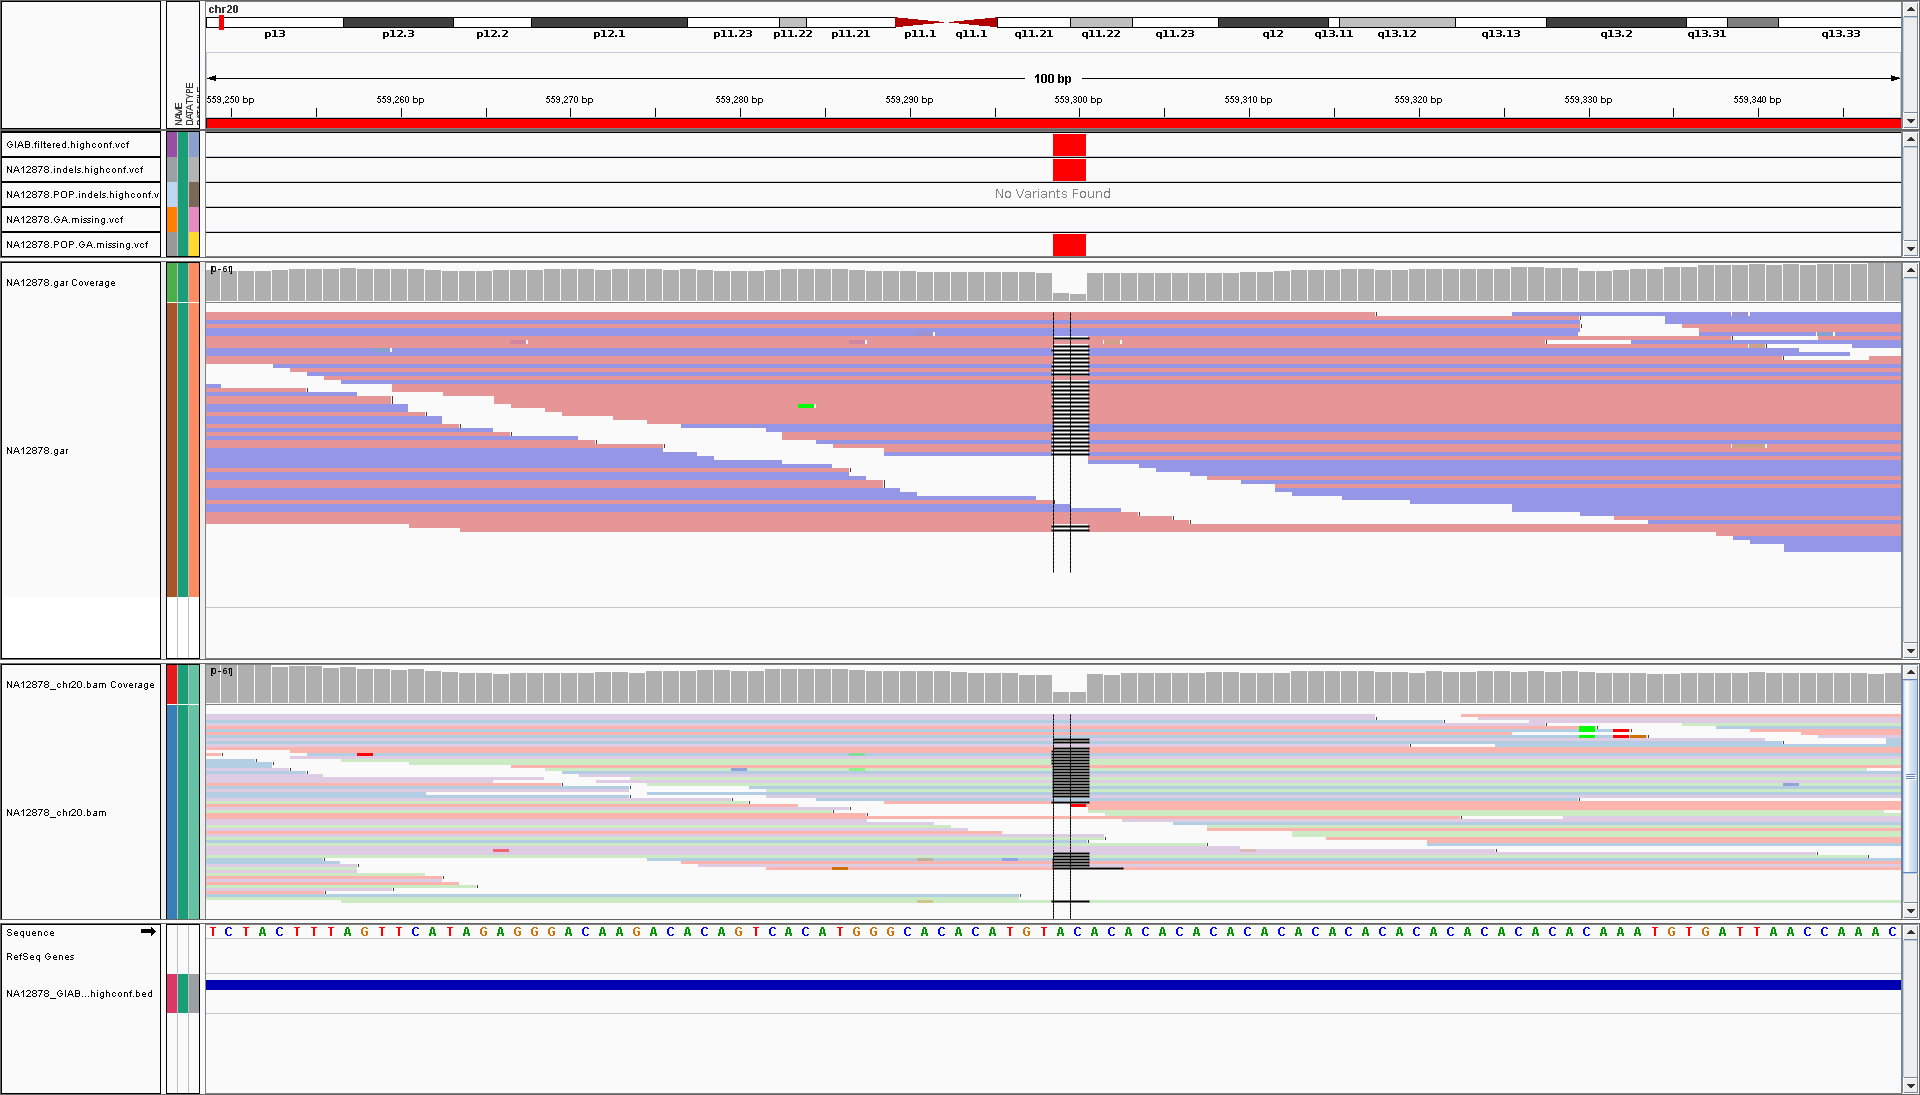
\includegraphics[width=1.0\linewidth]{missing_repeat_del.png}}
\end{frame}

\begin{frame}
\frametitle{Missing insert in repeat}
\center{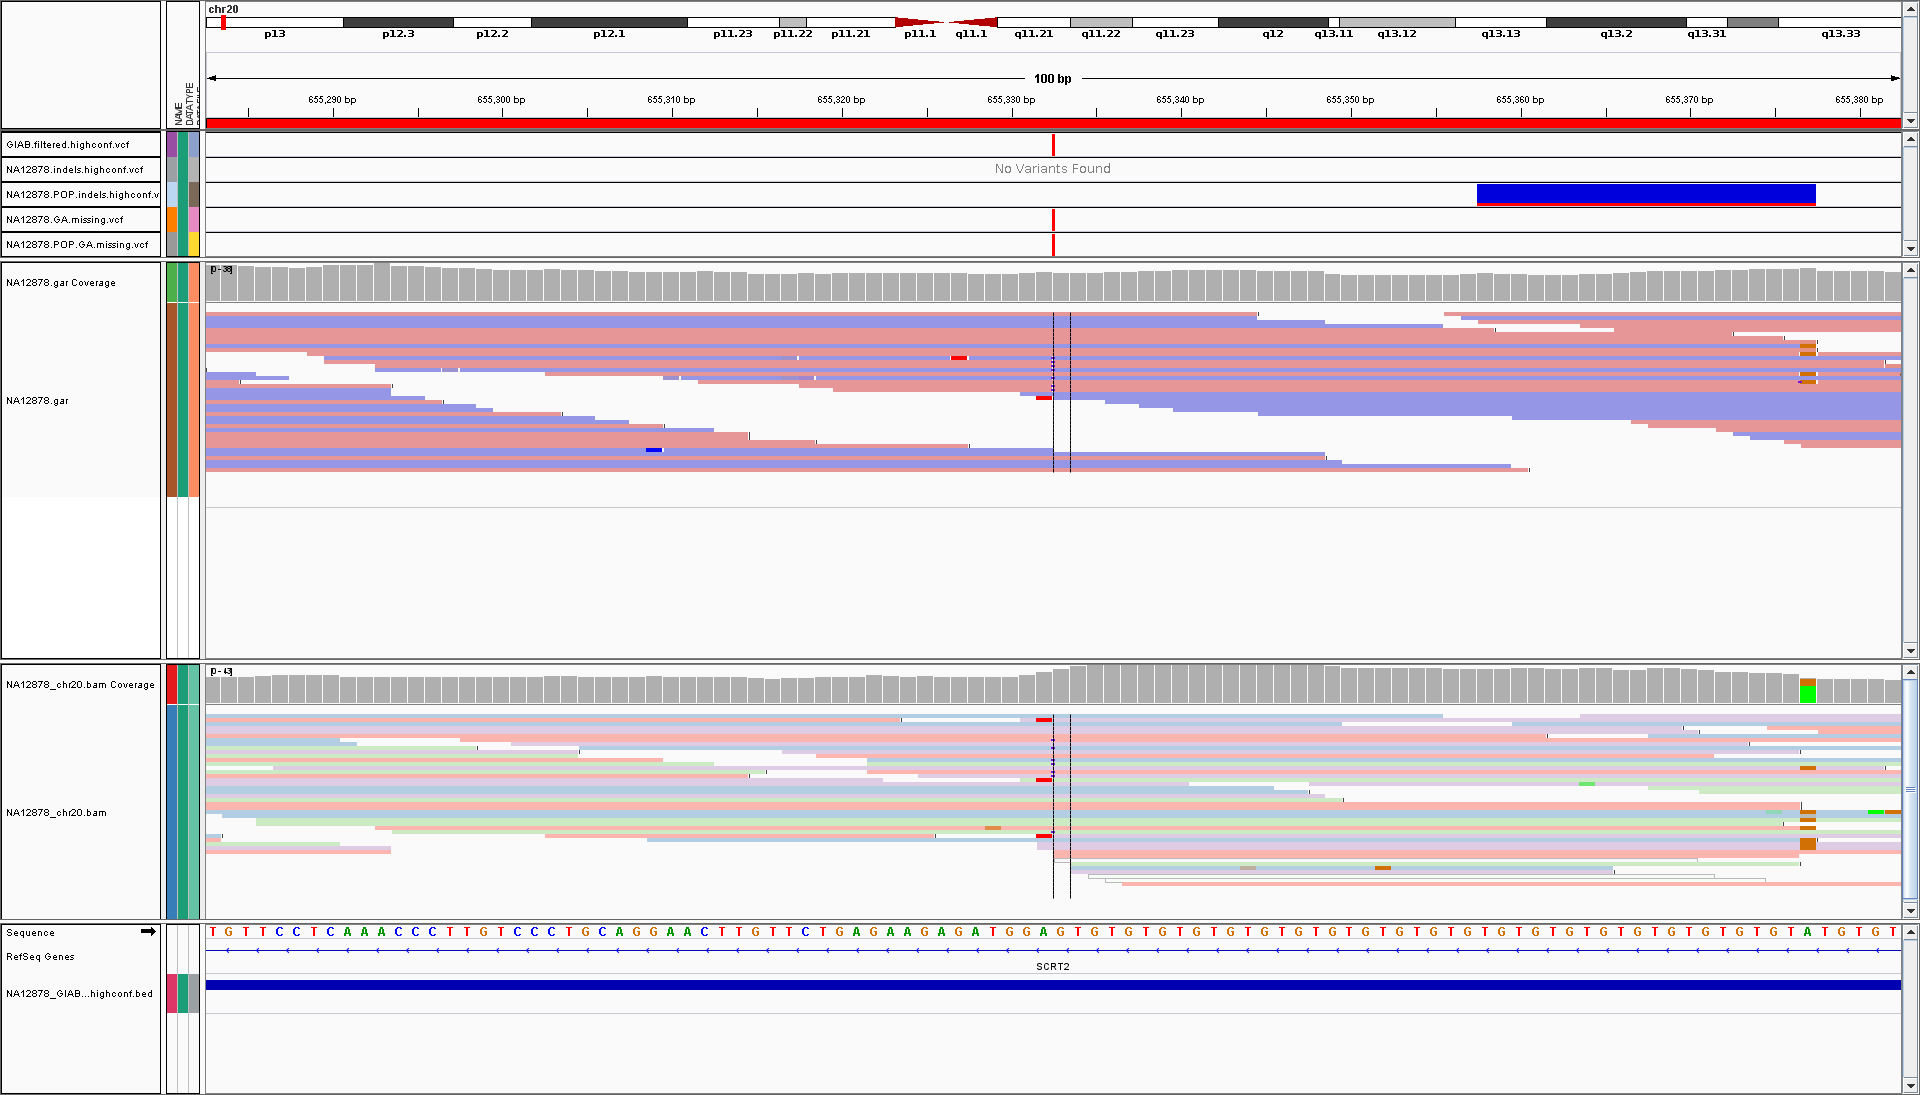
\includegraphics[width=1.0\linewidth]{missing_repeat_ins.png}}
\end{frame}

\begin{frame}
\frametitle{Resolution is different - not really missing}
\center{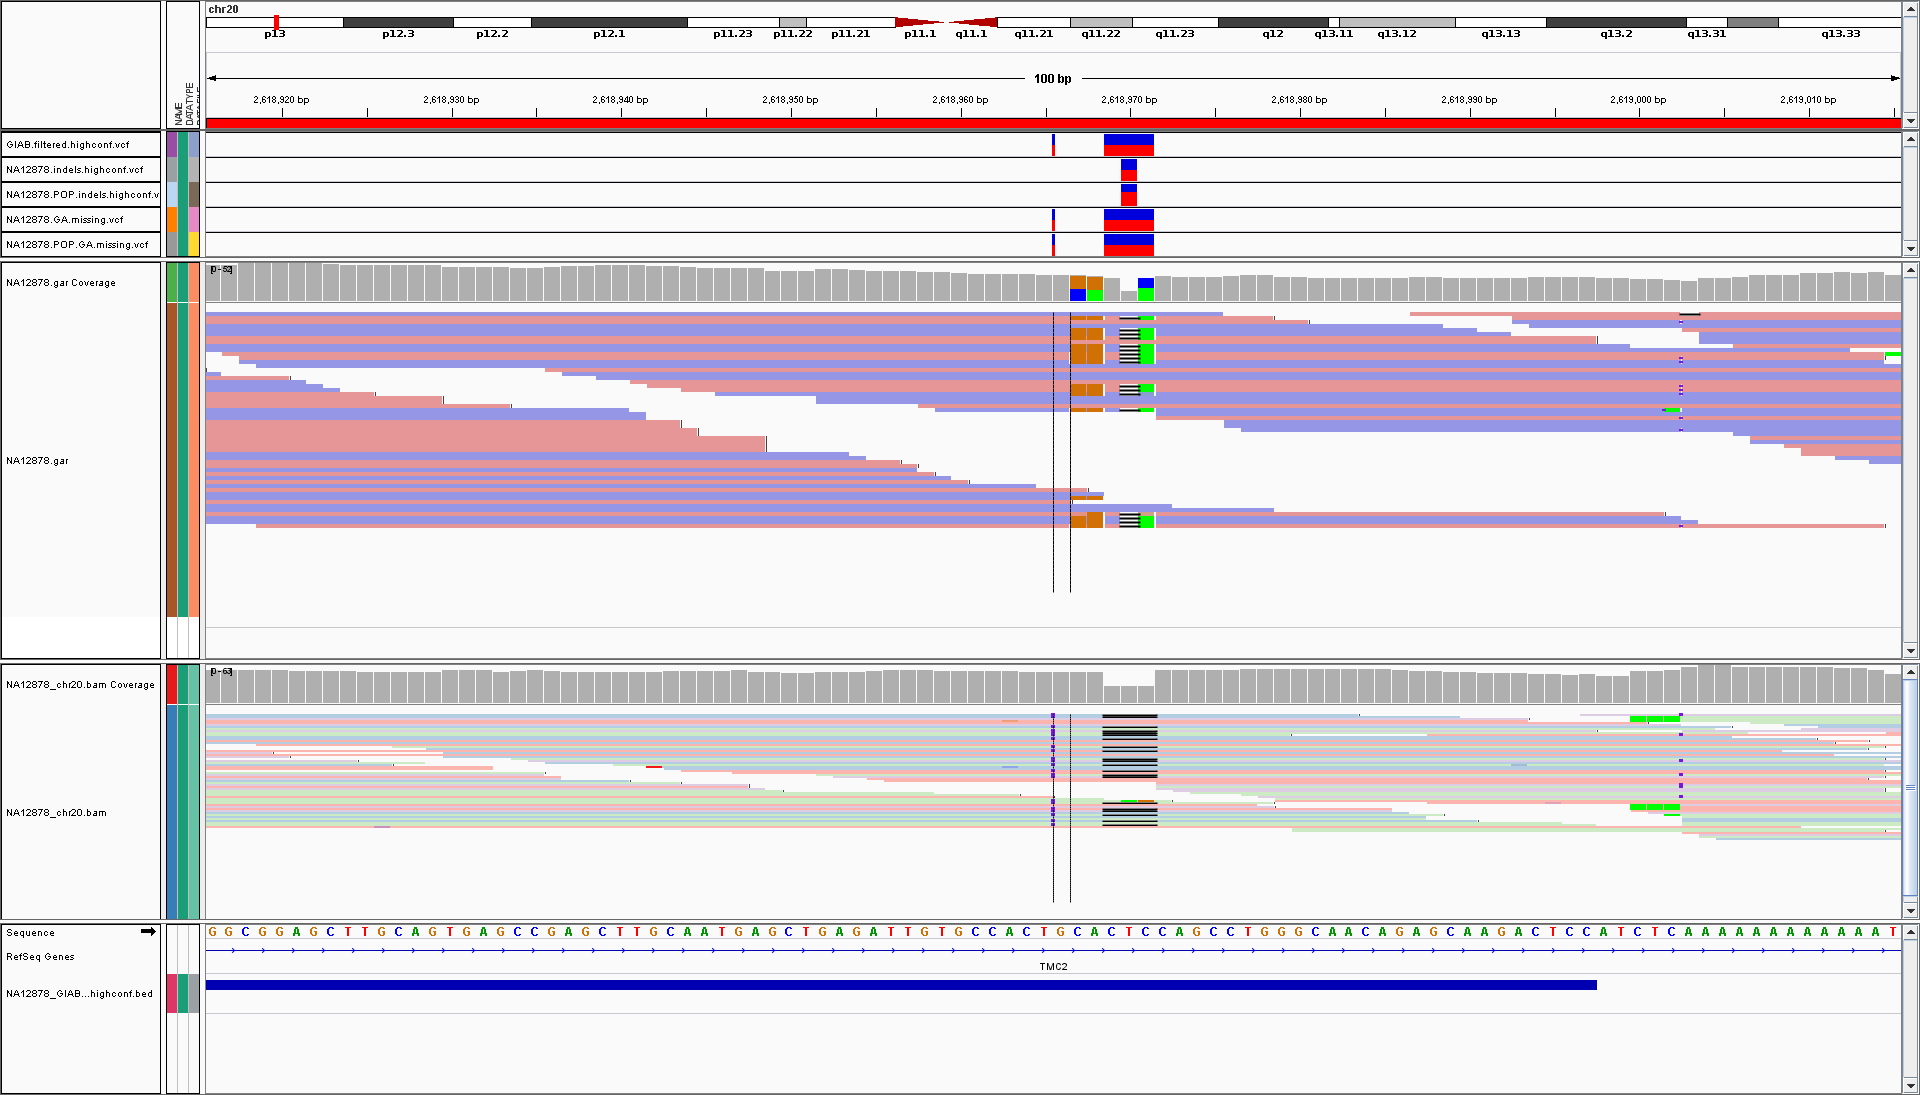
\includegraphics[width=1.0\linewidth]{different_resolution.png}}
\end{frame}

\begin{frame}
\frametitle{Yet an other missing insert}
\center{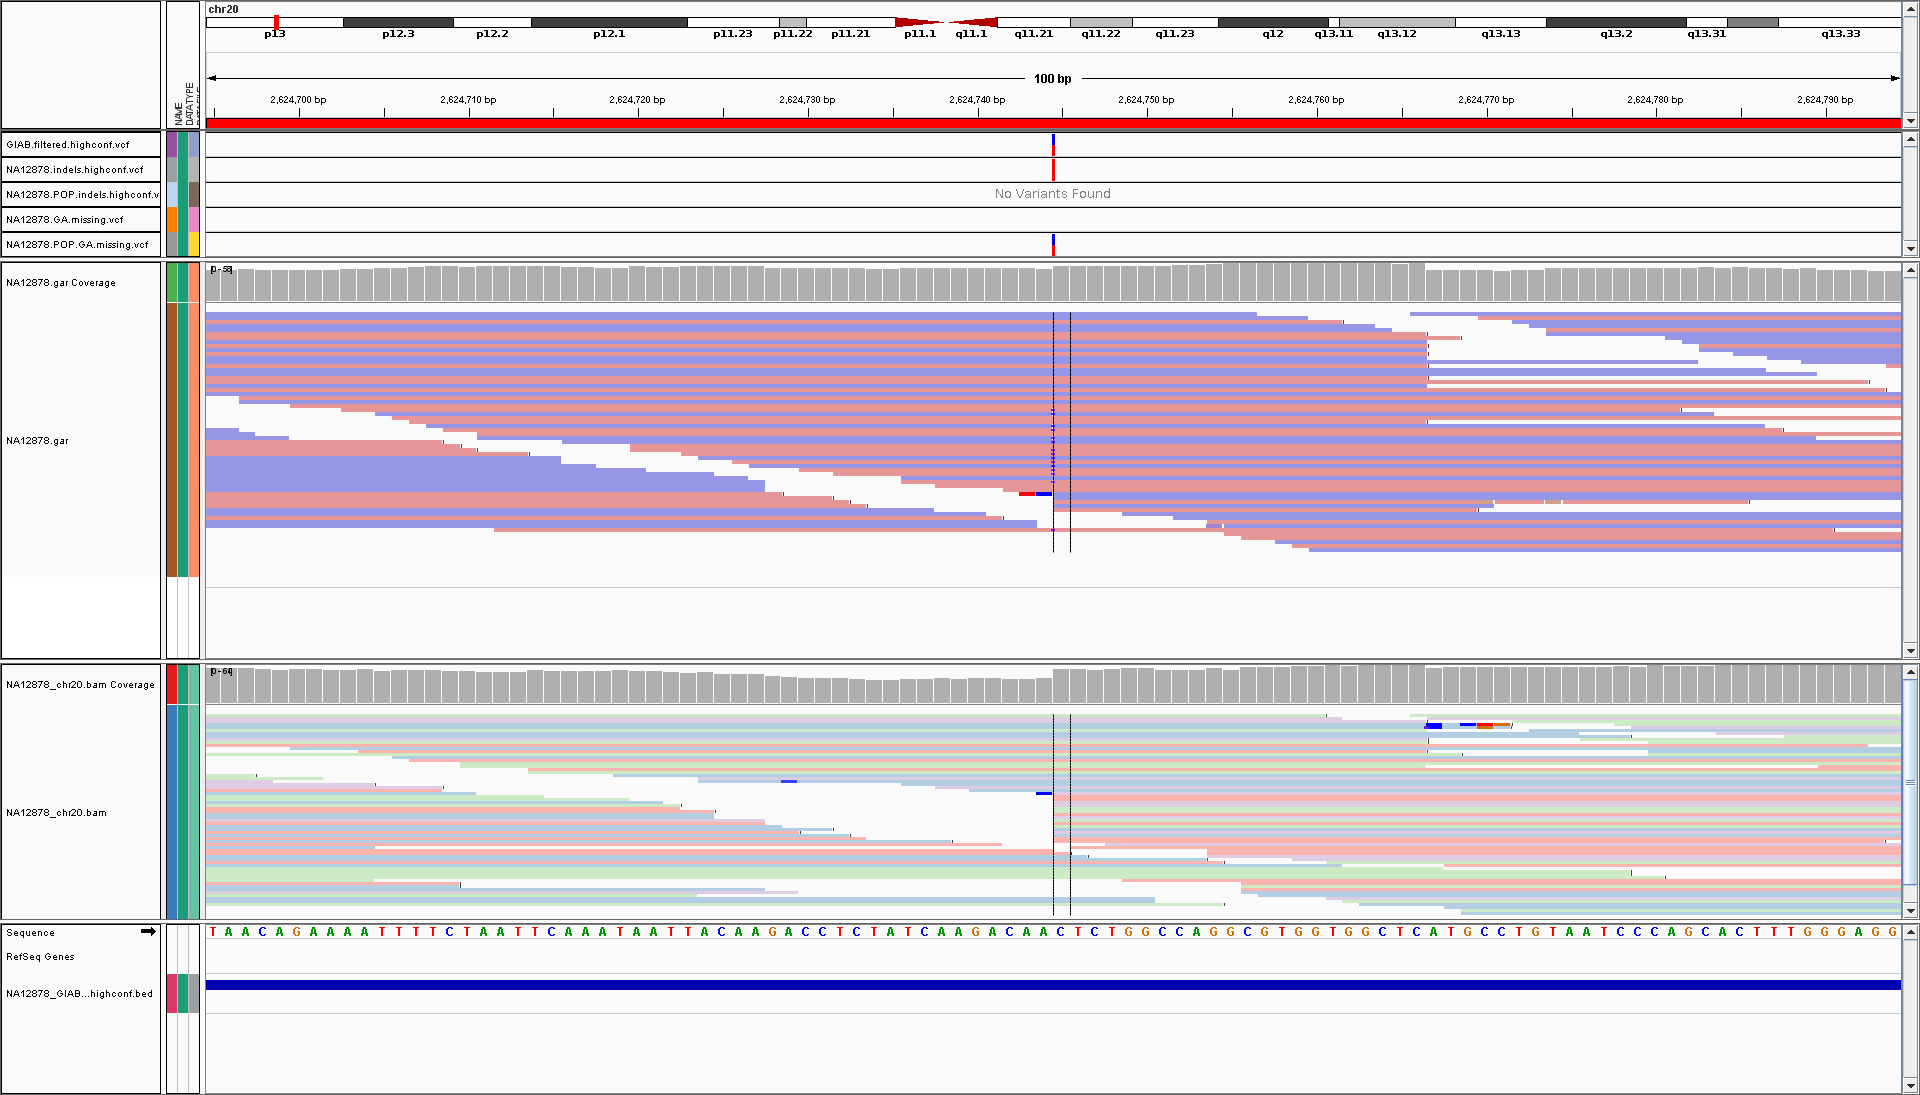
\includegraphics[width=1.0\linewidth]{missing_genuine_ins.png}}
The actual reads are reporting an insert, but the population caller is ignoring it - 
it is a CTCTGGCCAGGCGTGGTGGCTC insertion (repeat at insertion site)
\end{frame}

\begin{frame}
	\frametitle{Conclusions on indels}
	\begin{itemize}
		\item Missing indels are mostly at STRs or low-complexity regions
		\item There are extra indels not in the thruth set - yet to be analysed
		\item insert/deletion size distribution is very similar to the truth set
	\end{itemize}
	\begin{block}{TODO}
		\begin{itemize}
			\item Fire up NAS to test population calls
			\item Find indels and SNPs that are not in the truth set and looks like real calls 
		\end{itemize}
	\end{block}
\end{frame}

\end{document}
